% Chapter Template

\chapter{Introduction} % Main chapter title

\label{Chapter1} % Change X to a consecutive number; for referencing this chapter elsewhere, use \ref{ChapterX}

%-------------------------------------------------------------------------------------
%	INTRODUCTION
%-------------------------------------------------------------------------------------

Oxidation and reduction (redox) reactions play a vital role in biology. These reactions are characterized by a flow of electrons between chemical species. The species gaining electrons is said to have been oxidized, while the species losing electrons is said to have been reduced. Redox reactions are well-known to be involved in cellular respiration and metabolism more generally. More recently, redox control of the proteome has been the subject of great interest, mediating such events as differentiation and apoptosis \cite{circu2010}. The oxidation of cysteine thiols to disulfide bonds provides an interface between redox chemistry and proteomic signal transduction \cite{meyer2010}.

Many chemical species in the cell may exist in either an oxidized or reduced form. These pairs, termed \textit{redox couples} facilitate electron transfer in a variety of cellular processes. The \ce{NADH}/\ce{NAD+} couple, for example, transfers high energy electrons wrought from the oxidation of sugars in the citric acid cycle to \ce{O2} via oxidative phosphorylation.

% The tripeptide glutathione (GSH/GSSG in its reduced/oxidized form) is thought to play a particularly important role in the redox environment of the cell. It exists at high concentrations (1-11 mM), and is believed to act as a central hub in the network of cellular redox reactions.

The healthy cell actively maintains a steady-state disequilibrium of each of these redox couples. The "redox hypothesis" attributes aging and age-related disease to the misregulation of this network \cite{jones2008}. Quantifying redox chemistry in live cells will allow for a deeper understanding of the regulatory mechanisms that mediate these vital processes.

%-------------------------------------------------------------------------------------
%	SECTION 1
%-------------------------------------------------------------------------------------
\section{Fluorescent biomarkers enable real-time quantification of cytosolic protein oxidation} \label{fluorescenceIntro}
In a previous paper, our lab demonstrated the use of the genetically-encoded redox-sensitive fluorescent protein roGFP1\_R12 to quantify the cytosolic reduction potential in the pharyngeal muscle of \textit{C. elegans} in real-time \cite{romero-aristizabal2014}. These redox biosensors are leading to quantitative and mathematical models of the genetics and dynamics of intracellular and organismal-level redox signaling.

A key feature of the roGFP family of sensors is their ratiometric nature, which corrects for differential expression of the sensor, as well as cell thickness \cite{hanson2004}. Because the oxidized and reduced form of the protein have differing emission spectra, the emission intensity at differing excitation wavelengths may be used as estimates of concentration in the Nernst equation to determine the sensor's reduction potential \cite{meyer2010}. Thanks to the transparent nature of \textit{C. elegans}, fluorescence micrographs reveal spatial reduction potentials at subcellular resolution (Figure \ref{fig:ratioImageToE}).

\begin{figure}[ht]
    \centering
    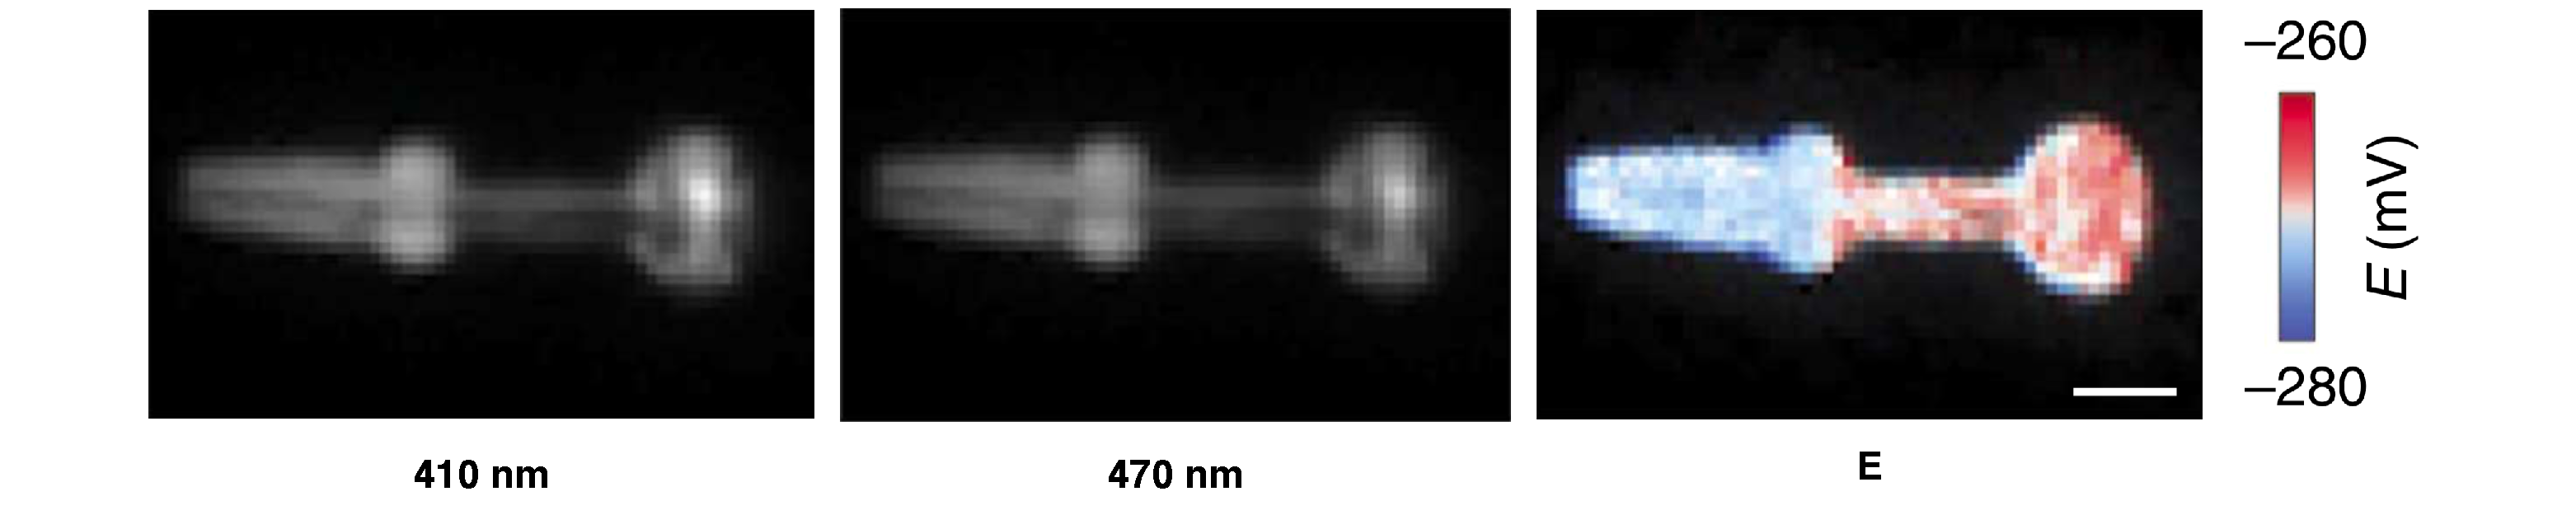
\includegraphics[scale=.25]{Figures/rendered_files/ratios_to_e}
    \decoRule
    \caption[Ratios of images to reduction potential]{Pixel-by-pixel ratios are transformed into redox potentials revealing a spatial pattern, adapted from \cite{romero-aristizabal2014}}
    \label{fig:ratioImageToE}
\end{figure}

Due to the cellular architecture of the pharynx, almost all of the variation in reduction potential follows the posterior-anterior axis. Thus, we can model the pharynx 1-dimensionally as the reduction potential along its posterior-anterior axis without losing significant information. Computationally, this is achieved by (1) estimating the centerline of the pharynx then (2) measuring the intensity of the images under this estimated centerline.

As will be discussed, a fundamental limitation of this analysis arises when the animal moves in the time between capturing the first and second frame in the pair of images required for each animal. 

%-------------------------------------------------------------------------------------
%	SECTION 2
%-------------------------------------------------------------------------------------
\section{Limitations of current pipeline} \label{limitations}
\subsection{Inter-frame movement results in measurement error} \label{limitationMovement}

The pharynx of \textit{C. elegans} acts as the animal's feeding muscle. It contracts along its anterior-posterior axis, functioning as a pump to bring in food. This contraction poses a problem for ratiometric analysis. Ordinarily, dividing intensities pixel-by-pixel is appropriate because pixel-coordinates in both images capture the same point in physical space. If the animal moves, however, the same point in space is represented by different pixel coordinates in the first and second image. To understand  why, consider Figure \ref{fig:MovementCartoon}.


\begin{figure}[ht]
    \centering
    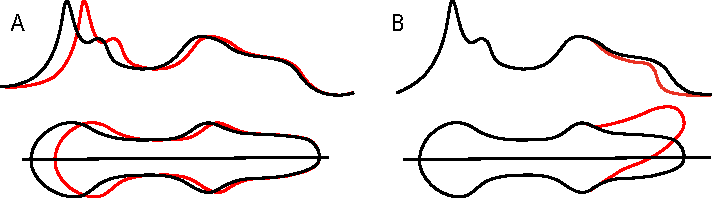
\includegraphics{Figures/rendered_files/movement_cartoon}
    \decoRule
    \caption[Pharyngeal contractions lead to boundary issues]{A cartoon shows the two most common modes of inter-frame movement. \textbf{A} Posterior bulb contractions lead to a shrink or stretch of the intensity profile. \textbf{B} Dorsal-ventral movement of the anterior tip leads to premature truncation of the intensity profile as the centerline does not follow the curve.}
    \label{fig:MovementCartoon}
\end{figure}

On the bottom we see the outline of the pharynx in each frame. The pharynx has contracted in one frame (red) and is elongated in the other (black). When the intensities along the posterior-anterior axis are plotted above, it is apparent that the contraction has lead to unwanted compression of the intensity profile.

Another common mode of inter-frame movement, dorsoventrally at the anterior tip, is represented similarly in Figure \ref{fig:MovementCartoon}. Dorsoventral anterior tip movements result in a loss of information about the tip in one frame, as depicted in red.

During imaging, animals are paralyzed with the acetyl choline agonist levamisole. However, complete paralysis is not currently possible. Inter-frame movement is currently addressed by visually screening the the ratio images for a highly textured appearance, as shown in Figure \ref{fig:HighMovement}. These animals are then excluded from analysis. However, visual screening is a time-intensive process, requires training, and is subject to experimenter error and bias.

\begin{figure}[ht]
    \centering
    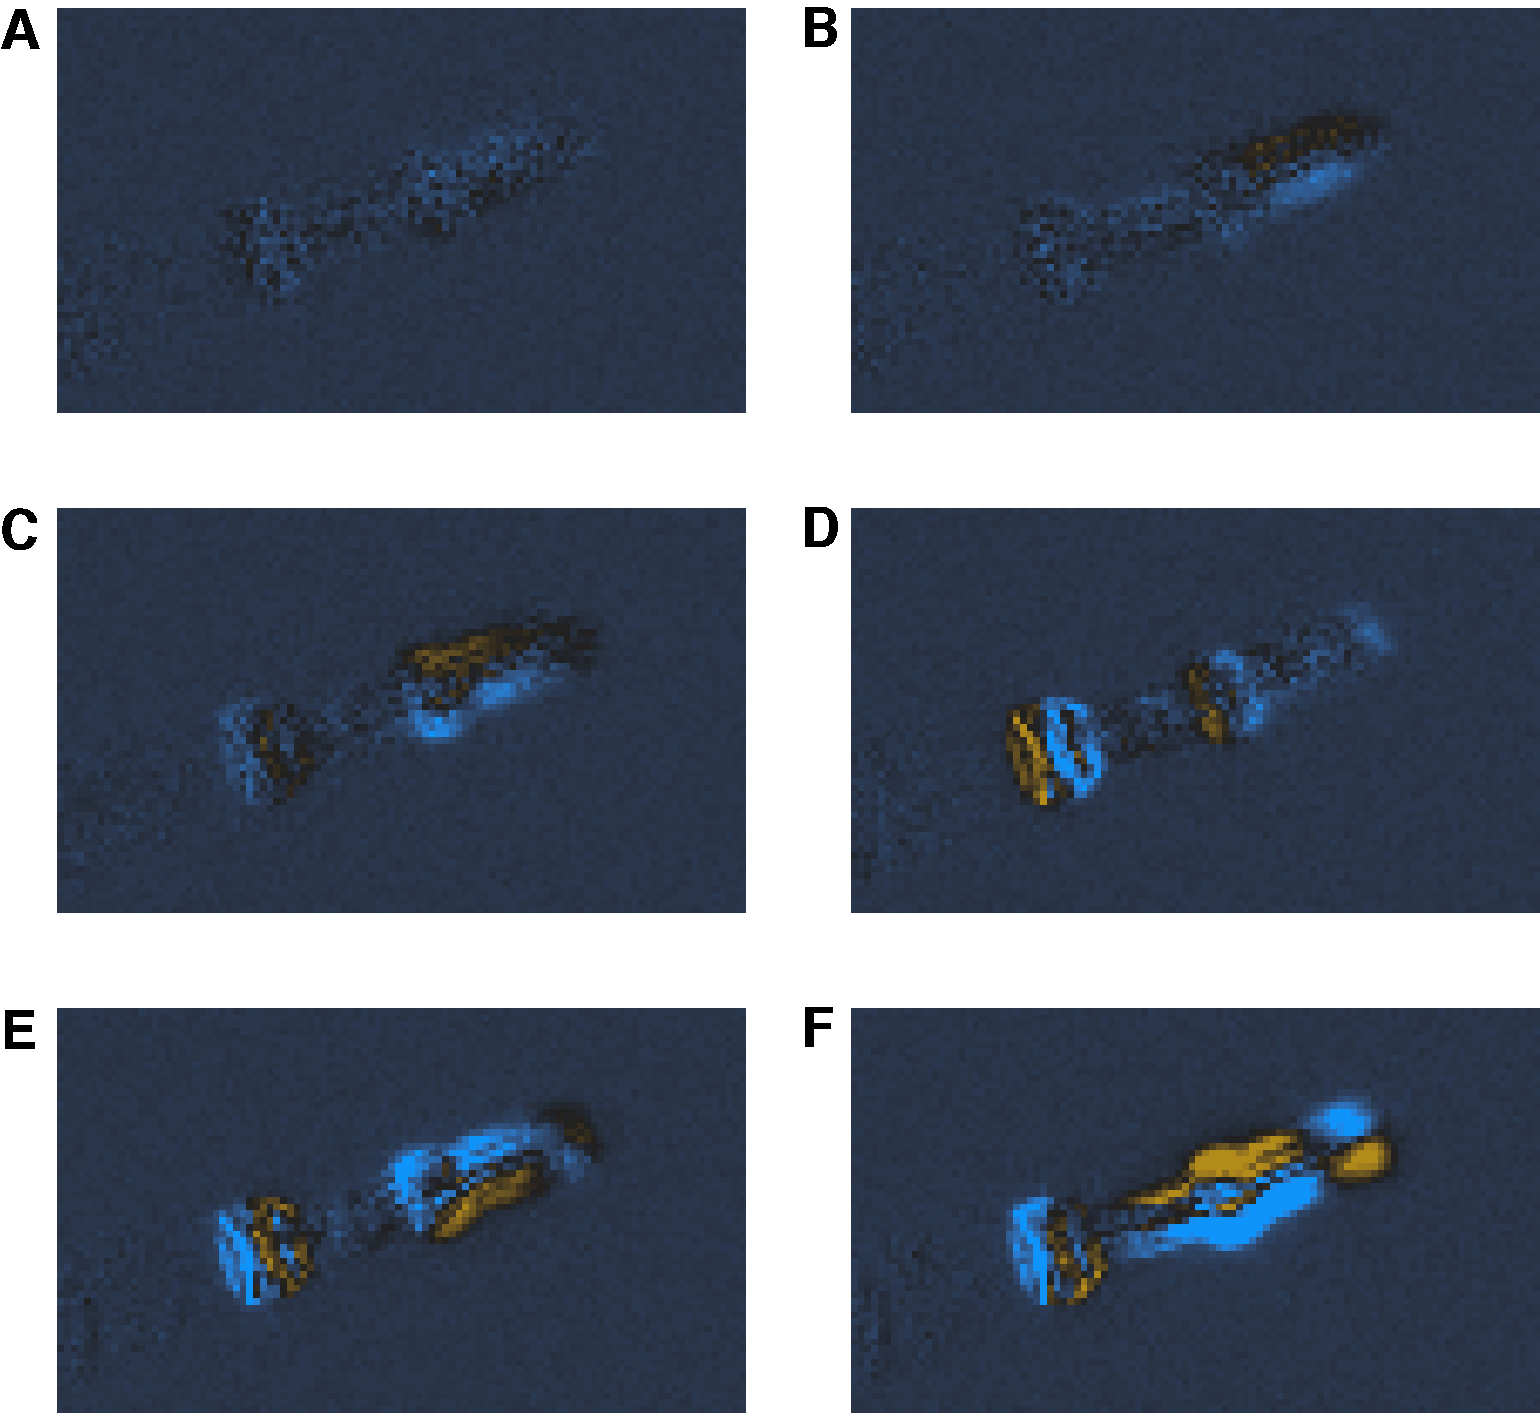
\includegraphics[scale=0.5]{Figures/rendered_files/movement_difference_images}
    \decoRule
    \caption[Difference images reveal movement]{Signed difference images reveal inter-frame movement. Each image depicts the signed difference between the first and second image in a pair taken at $\lambda = 410 \text{ nm}$, colored using a perceptually-uniform diverging colormap, CET-D6 \cite{kovesi2015}. \textbf{A} a pair with minimal inter-frame movement. This pair is considered ideal. \textbf{B} a pair with a small amount of dorsoventral around the anterior tip. \textbf{C} a pair with a moderate amount of dorsoventral anterior movement \textbf{D} a pair with a substantial shift along the posterior-anterior axis. \textbf{E} a pair with substantial contractions in the posterior bulb and dorsoventral anterior movement. \textbf{F} a pair with substantial contractions in the posterior bulb and dramatic anterior movement}
    \label{fig:HighMovement}
\end{figure}

\subsection{Segmentation and centerline estimation may require manual input} \label{limitationManual}

As noted, the visual screen for inter-frame movement is a manual step. Two other processes in the current pipeline also require manual supervision. The first is segmentation. Segmentation is the process by which pixels corresponding to objects in an image are given salient labels. In this case, the task is to separate the pharynx from everything else (Figure \ref{fig:SegmentationExample}). 

\begin{figure}[ht]
    \centering
    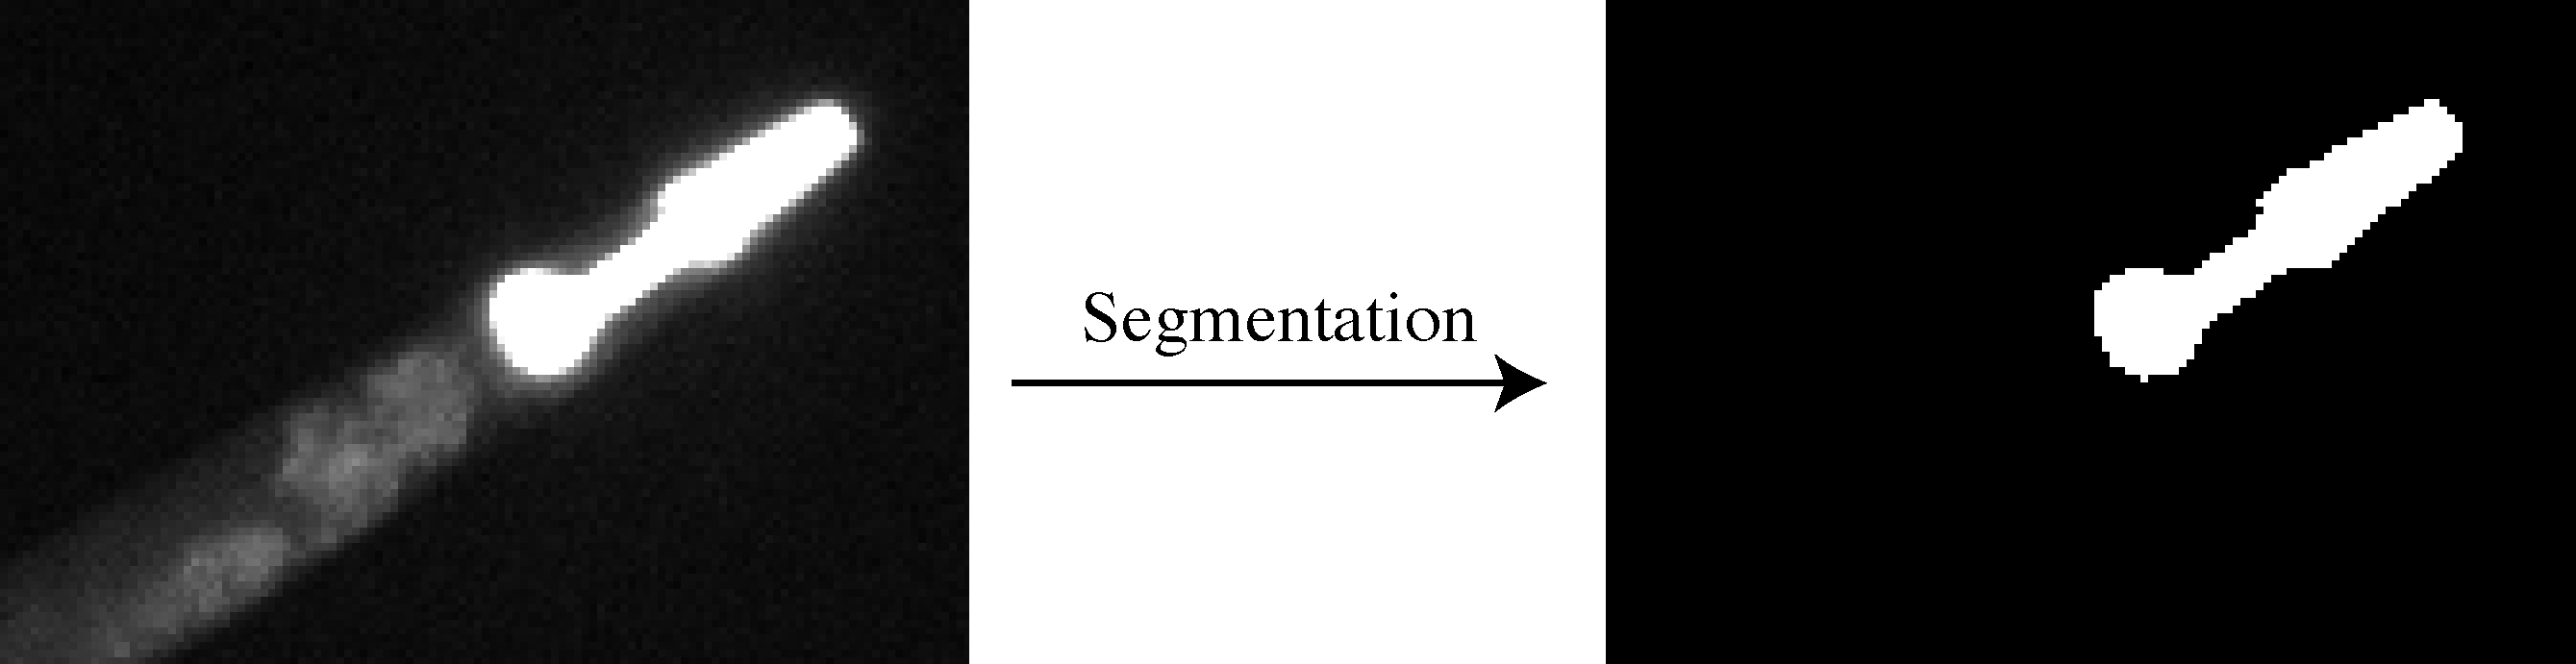
\includegraphics[scale=.25]{Figures/rendered_files/segmentation_description}
    \decoRule
    \caption[Segmentation of a fluorescence image]{The goal of segmentation. On the left, the original image showing fluorescence of roGFP in the pharynx and autofluorescence in the gut. On the right, a binary image consisting of value \texttt{1} in the pixels with a pharynx and value \texttt{0} elsewhere.}
    \label{fig:SegmentationExample}
\end{figure}

Because the transgenic animals express roGFP with pharynx-specific promoters, most fluorescence occurs only in the region of interest. However, the intestine of \textit{C. elegans} exhibits autofluorescence in response to the wavelengths of light required for roGFP excitation. This poses a problem for the static thresholding algorithm currently used to segment the pharynx. This algorithm assigns any value greater than a threshold the value \texttt{1} and those below the threshold \texttt{0}. Static thresholds work well when the distribution of brightness is different for each class of object in the image, but this is not the case when the intestine autofluoresces, resulting in ill-formed segmentation masks (Figure \ref{fig:SegmentationNaive}).

\begin{figure}[ht]
    \centering
    
\includegraphics[scale=.25]{Figures/rendered_files/segmentation_naive}
    \decoRule
    \caption[The problem with static thresholding]{The problem with static thresholding. Autofluorescent intestinal tissue results in a segmentation mask that must be manually corrected.}
    \label{fig:SegmentationNaive}
\end{figure}

As described in \ref{fluorescenceIntro}, the 1-dimensional model of the pharynx requires the accurate estimation of the tissue's centerline. While the current centerline estimation algorithm (described in \ref{Midlines}) works well in the interior regions of the pharynx, it is unstable around the terminal regions, both the anterior and posterior. These portions of the centerline must be visually inspected and corrected as well.

\section{Aims}
This thesis aims to address the limitations of the current analysis pipeline described in \ref{limitationMovement} and \ref{limitationManual}. To achieve this, a new pipeline was written in MATLAB to process and analyze these images end-to-end with little to no necessary manual input. The improved pipeline decreases the time required to analyze this data, standardizes the analysis, reduces human error, and mitigates movement-induced error.